\def\OPTIONConf{0}%
\def\OPTIONArxiv{0}%
%
\documentclass{llncs}
\usepackage{joshuadunfield}
\usepackage{boxedminipage}
\usepackage{goodcharter} %% XXX -- Check that ETAPS permits this font!
%\usepackage{euler}
\usepackage{mathtools}
\usepackage{semantic}   % Tools for typesetting PL semantics
\usepackage{braket}     % Easy angle-bracket notation
\usepackage{mathpartir} % Used to typeset blocks of inference rules
\usepackage{rotating} % for sidewaysfigure
%\usepackage{proof}
\usepackage{pdflscape}
\usepackage{fancyvrb} % to use \verb in footnotes
\usepackage{stmaryrd}
\let\proof\relax
\let\endproof\relax
\usepackage{amsmath,amsthm,amssymb}
%\usepackage{thmtools,thm-restate}

% Marvosym
\let\MathRightArrow\Rightarrow % save original definition of \Rightarrow
\usepackage{marvosym} % feloniously overrides \Rightarrow
\def\Rightarrow{\MathRightArrow}

%% \declaretheorem[style=mytheoremstyle]{theorem}
%% \declaretheorem[style=mytheoremstyle]{property}
%% %\declaretheorem[style=mytheoremstyle, sibling=theorem]{lemma}
%% \declaretheorem[style=mytheoremstyle]{lemma}
%% \declaretheorem[style=mytheoremstyle, sibling=lemma]{corollary}
%% \declaretheorem[style=mytheoremstyle, sibling=lemma]{conjecture}
%% \declaretheorem{example}
%% \makeatletter
%% \declaretheorem[style=mytheoremstyle, sibling=lemma, 
%% %             postheadhook={%
%% %               envname is `\thmt@envname'; %
%% %               thmname is `\thmt@thmname'; %
%% %               optarg is `\thmt@optarg'; %
%% %%               innercounters are `\thmt@innercounters'.
%% %             }
%%        ]{proposition}
%% \makeatother
%% \declaretheorem{remark}
%% \declaretheorem[style=mytheoremstyle]{definition}


%% \theoremstyle{remark}

\newcommand{\Label}[1]{\label{#1}} % XXX
\newcommand{\FLabel}[1]{\label{#1}} % XXX
\newcommand{\D}{\mathcal{D}}
\newcommand{\Ss}{\mathcal{S}}
\newcommand{\derives}{::}
\newcommand{\satisfactory}{~\textsf{satisfactory}}
%\newcommand{\wf}{~\textsf{wf}}

%% \newtheorem{thm}{Theorem}[section]
%% \newtheorem*{thm*}{Theorem}
%% \newtheorem{lem}[thm]{Lemma}
%% \newtheorem{conj}[thm]{Conjecture}
%% \newtheorem{prop}[thm]{Proposition}
%% \newtheorem*{cor}{Corollary}
%% \newcommand{\thmref}[1]{Theorem~\ref{thm:#1}}
%% \newcommand{\thmreftwo}[2]{Theorems \ref{thm:#1} and~\ref{thm:#2}}
%% \newtheorem{defn}[thm]{Definition}

\newcommand{\vUnit}{\texttt{()}}
\newcommand{\Unit}{\tyname{unit}}
\newcommand{\Nat}{\tyname{nat}}

\newcommand{\runonboldsf}{\sffamily\bfseries\selectfont}
\newcommand{\boldsf}[1]{\text{\runonboldsf #1}}

% ILC Computation types
\newcommand{\xF}{\boldsf{F}}
\newcommand{\xU}{\boldsf{U}}
\newcommand{\tyFp}[1]{\xF(#1)}
\newcommand{\tyF}[1]{\xF\,#1}
\newcommand{\tyUp}[1]{\xU(#1)}
\newcommand{\tyU}[1]{\xU\,#1}

% ILC Read and Write channel types
\newcommand{\xRd}{\boldsf{Rd}}
\newcommand{\tyRdp}[1]{\xRd(#1)}
\newcommand{\tyRd}[1]{\xRd\,#1}

\newcommand{\xWr}{\boldsf{Wr}}
\newcommand{\tyWr}[1]{\xWr\,#1}
\newcommand{\tyWrp}[1]{\xWr(#1)}

% ILC Modes
\newcommand{\Rm}{\textsf{R}} % read mode
\newcommand{\Wm}{\textsf{W}} % write mode
\newcommand{\Vm}{\textsf{V}} % value mode

% Currently, using \All for both type variables (\All{\alpha : K}
% and index variables (\All{ea : \sort})
\newcommand{\Allsym}{\forall}
\newcommand{\All}[1]{\Allsym{#1}.\,}

\newcommand{\Split}[4]{\keyword{split}\Lparen{#1}, {#2}.{#3}.{#4}\Rparen}
\newcommand{\Case}[5]{\keyword{case}\Lparen{#1}, {#2}.{#3}, {#4}.{#5}\Rparen}

\newcommand{\inj}[1]{\keyword{inj}_{#1}\,}
\newcommand{\Inj}[1]{\inj{#1}}

\newcommand{\vPair}[2]{\Lparen{#1}\texttt{,}{#2}\Rparen}
\newcommand{\vInj}[2]{\keyword{inj}_{#1}\Lparen#2\Rparen}
\newcommand{\vThunk}[1]{\keyword{thunk}\Lparen#1\Rparen}

\newcommand{\eSplit}[4]{\keyword{split}\Lparen{#1}, {#2}.{#3}.{#4}\Rparen}
\newcommand{\eCase}[5]{\keyword{case}\Lparen{#1}, {#2}.{#3}, {#4}.{#5}\Rparen}

\newcommand{\eFork}[2]{\ensuremath{#1 *&& #2}}
\newcommand{\eChoose}[2]{\ensuremath{#1 *|| #2}}



\newcommand{\Sig}{\mathcal{S}}

\newcommand{\xFork}{\mathrel{|\rhd}}

%% Math ligatures (thanks to the semantic package) that make it
%% easier to typeset math using readable LaTeX text.
%\mathlig{|-->}{\longmapsto}
\mathlig{::=}{\bnfas}
\mathlig{|}{\;|\;}
% \mathlig{[[}{\mbsf{[}}
% \mathlig{]]}{\mbsf{]}}
\mathlig{[[}{\texttt{\upshape[}}
\mathlig{]]}{\texttt{\upshape]}}
\mathlig{**}{\times}
\mathlig{|>}{\rhd}
\mathlig{->}{\arr}
\mathlig{-->}{\rightarrow}
\mathlig{--->}{\longrightarrow}
\mathlig{=>}{\Rightarrow}
\mathlig{*!}{\boldsf{!}}
\mathlig{||}{\mathrel{|\!|}}
\mathlig{;;}{\mathrel{;}}
\mathlig{*&&}{\mathrel{\xFork}}
\mathlig{*||}{\mathrel{\oplus}}

\mathlig{@>}{\arr_{\namesort}}


\newcommand{\eff}[2]{{#1} |> {#2}}
\newcommand{\effseqsym}{\mathsf{then}}
\newcommand{\effseq}{\,\effseqsym\,}

\newcommand{\effcoalsym}{\mathsf{after}}
\newcommand{\effcoal}{\,\effcoalsym\,}

\newcommand{\Lparen}{\texttt{(}}
\newcommand{\Rparen}{\texttt{)}}
% \newcommand{\Pair}[2]{\Lparen{#1}\texttt{,}{#2}\Rparen}


%\mathlig{unit}{\unitty}


% Bidirectional typing

\newcommand{\chkcolor}{dBlue}
\newcommand{\syncolor}{dRed}
\newcommand{\isyncolor}{dGreen}
\newcommand{\chk}{\mathrel{\mathcolor{\chkcolor}{\Leftarrow}}}
\newcommand{\uncoloredsyn}{{\Rightarrow}}
\newcommand{\syn}{\mathrel{\mathcolor{\syncolor}{\uncoloredsyn}}}
\newcommand{\RRightarrow}{\mathrel{\mathrlap{\Rightarrow}\mkern2mu\Rightarrow}}
\newcommand{\isyn}{\mathrel{\mathcolor{\isyncolor}{\RRightarrow}}}
\mathlig{<<}{\langle}
\mathlig{>>}{\rangle}
\mathlig{==>}{\syn}
\mathlig{<==}{\chk}
%\mathlig{||}{\Downarrow}
\mathlig{!!}{\Downarrow}
% \mathlig{..}{\epsilon}

\newcommand{\e}{\epsilon}
\newcommand{\hist}{\mathcal{H}}

\newcommand{\ambns}{M}

\newcommand{\disjoint}{\mathrel{\bot}}

\newcommand{\tbrack}[1]{\texttt{\upshape[}{#1}\texttt{\upshape]}}

\newcommand{\rootname}{\textvtt{root}}

%\newcommand{\tv}{tv}
\newcommand{\Mv}{V}
\newcommand{\ntevalsym}{\Downarrow_{\mathsf{M}}}
\newcommand{\nteval}{\mathrel{\ntevalsym}}

\newcommand{\xrefv}{\keyword{ref}}
\newcommand{\xthunk}{\keyword{thunk}}
\newcommand{\xunthunk}{\keyword{unthunk}}
\newcommand{\xname}{\keyword{name}}
%\newcommand{\xName}{\tyname{Name}}
\newcommand{\xName}{\tyname{Nm}}

\newcommand{\xRef}{\tyname{Ref}}
%\newcommand{\xThunk}{\tyname{Thunk}}
\newcommand{\xThunk}{\tyname{Thk}}
\newcommand{\xUnthunk}{\tyname{Unthunk}}

\newcommand{\refv}[1]{\xrefv\;{#1}}
\newcommand{\thunk}[1]{\xthunk\;{#1}}
\newcommand{\unthunk}[1]{\xunthunk\;{#1}}
\newcommand{\name}[1]{\xname\;{#1}}
\newcommand{\Name}[1]{\xName\tbrack{#1}}


\newcommand{\Ref}[1]{\xRef\tbrack{#1}\,}
\newcommand{\Thk}[1]{\xThunk\tbrack{#1}\,}
\newcommand{\Unthk}[1]{\xUnthunk\tbrack{#1}\,}
\newcommand{\Thunk}[2]{\keyword{thunk}\Lparen{#1},{#2}\Rparen}
\newcommand{\Unthunk}[1]{\keyword{unthunk}\Lparen{#1}\Rparen}
\newcommand{\Refe}[2]{\keyword{ref}\Lparen{#1},{#2}\Rparen} % Ref expression form

\newcommand{\List}[3]{\tyname{List}\tbrack{#1;#2}~{#3}}
\newcommand{\Art}[2]{\tyname{Art}\tbrack{#1}~{#2}}
\newcommand{\Int}[0]{\tyname{Int}}

\let\Force\undefined
\newcommand{\eForce}[1]{\keyword{force}\Lparen{#1}\Rparen}

\newcommand{\App}[2]{#1\,#2}
\newcommand{\eApp}[2]{#1\,#2}

\newcommand{\Ret}[1]{\keyword{ret}\Lparen{#1}\Rparen}
\newcommand{\Let}[3]{\keyword{let}\Lparen{#1},{#2}.{#3}\Rparen}
\newcommand{\eLet}[3]{\keyword{let}\Lparen{#1},{#2}.{#3}\Rparen}
\newcommand{\LetBang}[3]{\keyword{let!}\Lparen{#1},{#2}.{#3}\Rparen}

% Channel read and Channel write expressions
\newcommand{\eRd}[1]{\keyword{rd}\Lparen#1\Rparen}
\newcommand{\eWr}[2]{\keyword{wr}\Lparen#1<-#2\Rparen}
\newcommand{\eNu}[2]{\nu#1.\,#2}

\newcommand{\xstoretype}{\textsf{has-store-type}}
\newcommand{\storetype}{\;\xstoretype\;}

\newcommand{\xterminal}{\textsf{terminal}}
\newcommand{\terminal}{\;\xterminal}

\newcommand{\Config}[2]{\left<#1;#2\right>}

\newcommand{\Chans}{\Sigma}
\newcommand{\vChan}[1]{\texttt{chan}\Lparen#1\Rparen}
\newcommand{\emptyChans}{\varepsilon}

\newcommand{\emptyctxt}{\cdot}

\newcommand{\Procs}{\pi}
\newcommand{\proc}{e}
\newcommand{\emptyProcs}{\varepsilon}

\newcommand{\bnfheader}[1]{\multicolumn{4}{@{}l}{\text{#1}}}
\newenvironment{sbnfarray}{\begin{tabular}{c}\begin{array}[t]{lr@{~~}c@{~~~}ll}}{\end{array}\end{tabular}}
\newenvironment{bnfarray}{\begin{tabular}{c}\begin{array}[t]{r@{~~}c@{~~~}ll}}{\end{array}\end{tabular}}
\newenvironment{xbnfarray}{\begin{tabular}{c}\begin{array}[t]{r@{~~}c@{~}l@{~~}l}}{\end{array}\end{tabular}}

\newcommand{\DHasEffects}[3]{#1~\textsf{reads}~#2~\textsf{writes}~#3}
\newcommand{\DByHasEffects}[4]{#1~\textsf{by}~#2~\textsf{reads}~#3~\textsf{writes}~#4}
\newcommand{\mergeRds}{\cup}
\newcommand{\joinWrs}{\mathrel{\ast}}
\newcommand{\joinGrs}{\mathrel{\ast}}
\newcommand{\mergeGrs}{\cup}
\newcommand{\restrict}[2]{\textsf{restrict}\lfloor{#1}\rfloor_{#2}}
\newcommand{\dom}[1]{\textsf{dom}(#1)}
\newcommand{\update}[4]{#1\{#2 \mapsto #3\} = #4}
%\newcommand{\disjoint}{\cupplus}

%\newcommand{\Dee}{\mathcal{D}}
%\newcommand{\D}{\mathcal{\Dee}}

\newcommand{\te}{e_{\mathsf{terminal}}}

\newcommand{\nfap}[3]{{\color{blue}{}^{#1}_{#2}}{\color{blue}\big[} #3 {\color{blue}\big]}}

%%% Local Variables: 
%%% mode: latex
%%% TeX-master: types
%%% End: 

\newcommand{\msf}[1]{\ensuremath{{\mathsf {#1}}}}
\newcommand{\mtt}[1]{\ensuremath{\mathtt {#1}}}
\newcommand{\mcal}[1]{\ensuremath{\mathcal {#1}}}
\newcommand{\val}{\msf{val}}
\newcommand{\sn}{\msf{sn}}

\newcommand{\tn}{\textnormal}
\newcommand{\codeb}[1]{\textsf{#1}}
\newcommand{\hash}{\ensuremath{{\cal H}}}
\newcommand{\adv}{\ensuremath{{\mathcal A}}\xspace}
\newcommand{\Adv}{\adv}
\newcommand{\A}{\adv}
\newcommand{\samples}{\overset{\$}{\leftarrow}}
\newcommand{\SA}{\msf{SA}}
% SaUCy specific
\newcommand{\SaUCy}{\xspace{\msf{SaUCy}}\xspace}
\newcommand{\leak}{\color{blue}\mtt{leak}}
\newcommand{\eventually}[1]{\color{blue}\mtt{leak}}
\newcommand{\poly}{\textnormal{poly}}
\newcommand{\negl}{\textnormal{negl}}
\newcommand{\execUC}[4]{\mtt{execUC}({#1},{#2},{#3},{#4})}
\newcommand{\chan}[1]{{\underline{\smash{\msf{#1}}}}}
\newcommand{\functionality}[1]{\ensuremath{{\cal F}_{\textnormal{\msf{{#1}}}}}}
\newcommand{\F}{\functionality}
\newcommand{\G}[1]{{\cal G}_{\textnormal{\tiny {\uppercase{#1}}}}}
\newcommand{\GG}[1]{{\overline {\cal G}}_{\textnormal{\tiny {\uppercase{#1}}}}}
\renewcommand{\C}[1]{{\cal C}_{\textnormal{\tiny {\uppercase{#1}}}}}
\renewcommand{\P}{\ensuremath{\mathcal P}}
\newcommand{\Ps}{\ensuremath{\{\mathcal{P}_i\}_{i \in [N]}}}
\renewcommand{\S}{\ensuremath{\mathcal S}}
\newcommand{\env}{\Z}
\newcommand{\Z}{{\mcal{E}}}
\newcommand{\R}{{\mathcal R}}

\usepackage{enumitem}

\newcommand{\mc}[1]{\mathcal{{#1}}}
\newcommand{\parheader}[1]{\noindent\emph{\textbf{{#1}.}}}

\title{SaUCy: Super Amazing Universal ComposabilitY}
\author{Kevin Liao}
\institute{}

\begin{document}

\maketitle

\begin{abstract}
\ldots
\end{abstract}

\section{Introduction}

Proving that a protocol is secure is an essential component in cryptographic
protocol design. To do so, we must rigorously define what security means, and
then demonstrate that the protocol lives up to the definition. First-cut security
definitions for cryptographic tasks consider only a standalone execution of the
protocol. While this simplifies analyses, these definitions are insufficient
when analyzing the protocol in more complex contexts. Extended security
definitions have been formulated to remedy these drawbacks, but are often
complex and ad hoc.

The Universal Composability (UC) framework by
Canetti~\cite{canetti2001universally} takes an alternative approach---it is a
general framework for reasoning about the security of practically any
cryptographic protocol in a unified and systematic way. The idea is to formulate
a security definition and analyze the protocol as in the standalone model, but
to additionally show that the protocol composes securely with arbitrary other
protocols, i.e.,\ the protocol is secure in \emph{any context}. The benefit of
composability is that complex, UC-secure protocols can then be modularly
constructed from smaller UC-secure ``building blocks''.

While universally composable security is a powerful guarantee, elaborating UC
proofs is highly nontrivial. They are notoriously complex and exist primarily as
``pen-and-paper'' proofs, which makes many of them essentially
unverifiable. Thus, the goal of this work is to place the UC framework on a
proper analytic foundation by developing computer-aided tools and techniques for
reasoning in the UC framework.\smallskip

\parheader{Contributions} The main contributions of this work are the
following:
\begin{enumerate}
\item We design and implement a programming language called the Interactive
Lambda Calculus (ILC for short) for constructing algorithmic entities within the
UC execution model.
\item We implement the UC execution model in ILC along with a ``library'' of
example algorithmic entities (ideal functionalities).
\item We build a compiler for translating ILC programs into
EasyCrypt~\cite{barthe2011computer} modules, which allows us to construct
cryptographic proofs using EasyCrypt's interactive theorem proving facilities.
\end{enumerate}

\parheader{Organization} We first provide background on the UC framework in Section~\ref{sec:background}.

\section{Background}\label{sec:background}

In the Universal Composability framework, the security of a protocol is
analyzed \emph{in vitro} as a standalone protocol for simplicity, but
security \emph{in vivo}, that is, in realistic settings where the protocol can
run concurrently with arbitrarily many (even adversarially controlled)
protocols, is guaranteed by showing that security is preserved under a general
composition operation on protocols.

Demonstrating that a protocol meets its security definition in the standalone
model goes back to the real/ideal paradigm introduced
in~\cite{goldreich1987play}. First, envision an \emph{ideal protocol} $\phi$
(running with parties $\phi_1, \ldots, \phi_n$) that is secure by definition for
carrying out a cryptographic task. In the ideal protocol, each party hands their
input to an incorruptible trusted party, called an \emph{ideal functionality}
$\mc{F}$. The ideal functionality then performs the task locally and hands to
each party their prescribed output. We can think of the ideal protocol as a
formal specification for the security requirements of the task.

Of course, in the real world, such a trusted party does not exist! Since a real
world protocol $\pi$ (running with parties $\pi_1, \ldots, \pi_n$) cannot rely
on the ideal functionality to carry out the task securely, we would like to show
that $\pi$ \emph{emulates} the ideal protocol $\phi$, which does rely on the
ideal functionality. Informally, we show this by proving that whatever
``damage'' any adversary $\mc{A}$ can do to break $\pi$, there exists an
adversary $\mc{S}$ (known as a simulated adversary, or simulator) that can do
the same ``damage'' to break $\phi$. However, since $\phi$ is secure by
definition, the ``damage'' done by $\mc{A}$ does not break the security of
$\pi$. We will begin to formalize this idea shortly.

The above setup is sufficient for proving security in the standalone model,
which allows for secure \emph{sequential} composition. However, to generalize
composition to the \emph{concurrent} setting, the UC framework includes an
additional entity known as the environment $\mc{Z}$. Intuitively, the
environment represents everything external to the protocol in consideration---it
can hand inputs to protocol parties and interact freely with the adversary throughout the
protocol execution. Essentially, the environment acts as an outside observer,
and its job is to determine whether it is interacting with the real world setup
or the ideal world setup by examining what ``damage'' an adversary can do to
break the protocol. Similar to the security definition described in the
standalone model, if no $\mc{Z}$ can distinguish between the real world setup
(with $\pi$ and $\mc{A}$) and the ideal world setup (with $\phi$ and $\mc{S}$),
then we say that $\pi$ \emph{UC-emulates} $\phi$ and is
thus \emph{UC-secure}. Figure~\ref{fig:uc-experiment} shows the real world and
ideal world setups in the UC experiment.

\begin{figure}[!htb]
\centering
\begin{minipage}{.5\textwidth}
  \centering
  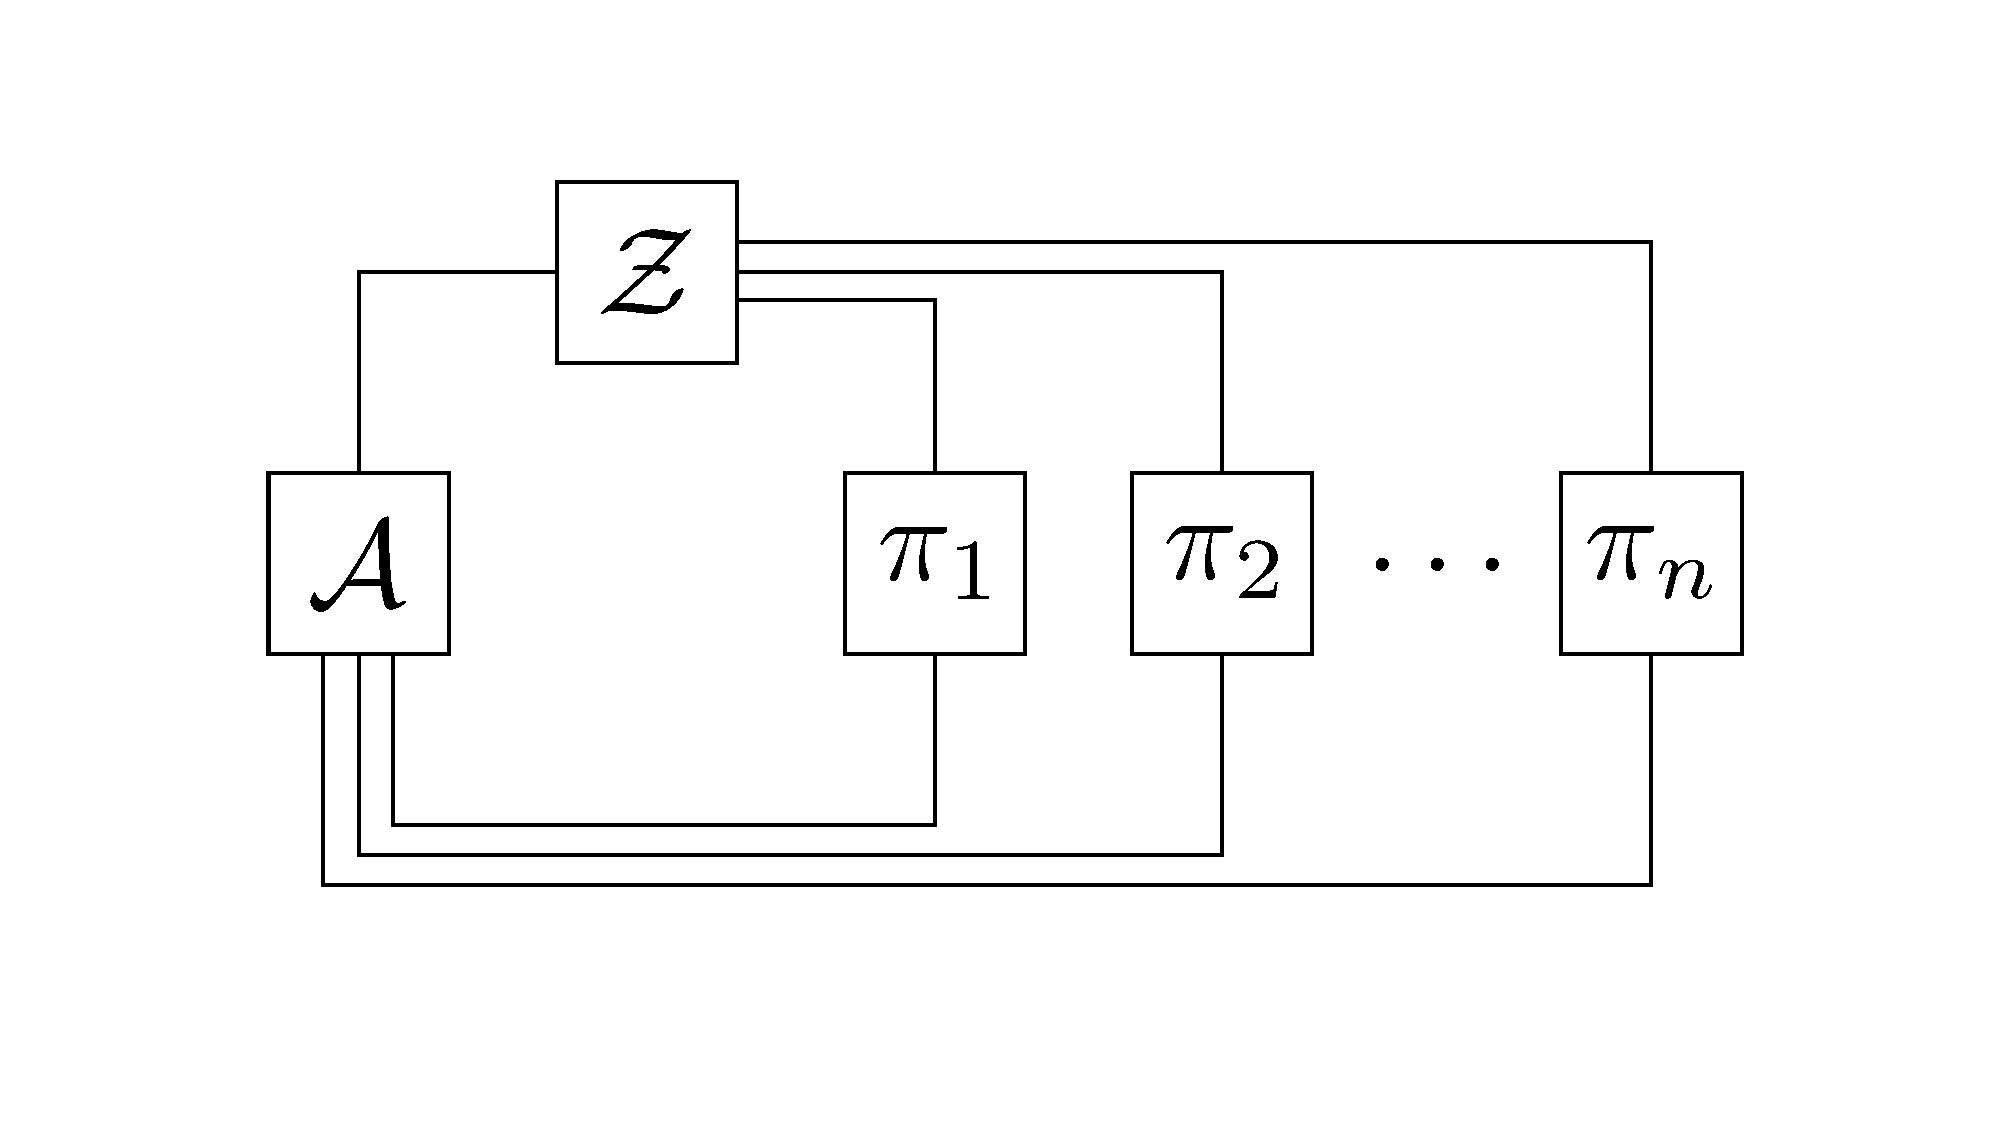
\includegraphics[width=0.8\textwidth]{real-setup}
\end{minipage}%
\begin{minipage}{.5\textwidth}
  \centering
  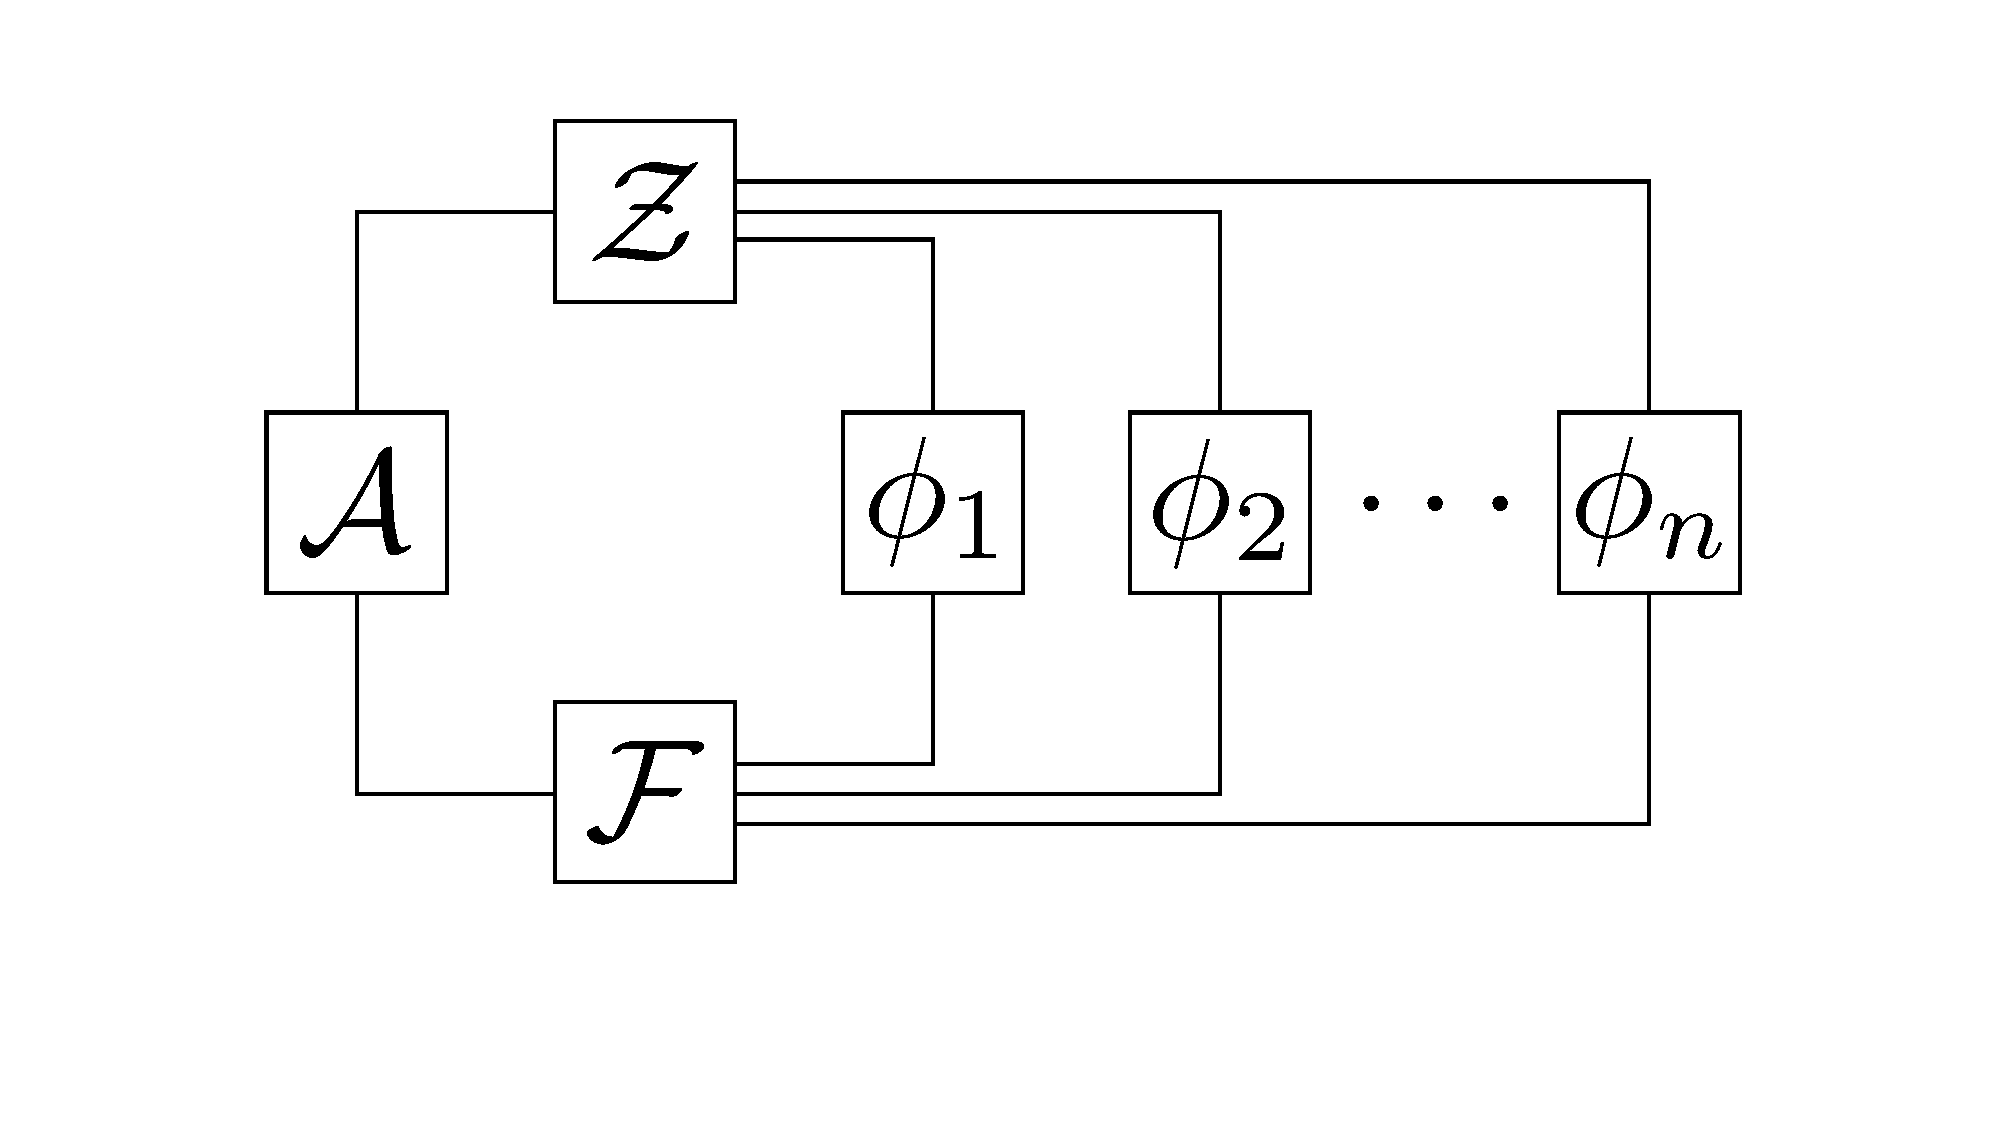
\includegraphics[width=0.8\textwidth]{ideal-setup}
\end{minipage}
\caption{Real world setup (left) and ideal world setup (right) in the UC experiment.}
\label{fig:uc-experiment}
\end{figure}

Having described the two setups in the UC experiment, we define the random
variable $\textsc{EXEC}_{\pi, \mc{A}, \mc{Z}}$ to be the output of $\mc{Z}$ in
the real world execution and the random variable
$\textsc{EXEC}_{\phi, \mc{S}, \mc{Z}}$ to be the output of $\mc{Z}$ in the ideal
world execution. Additionally, let $k$ be a security parameter.

\begin{definition}[UC Protocol Emulation]
Let $\pi$ and $\phi$ be protocols. We say that $\pi$ UC-emulates $\phi$ if for
any adversary $\mc{A}$ there exists an
adversary $\mc{S}$ such that for any environment $\mc{Z}$, we have:
\begin{equation*}
\textsc{EXEC}_{\phi, \mc{S}, \mc{E}} \approx \textsc{EXEC}_{\pi, \mc{A}, \mc{E}},
\end{equation*}
\noindent i.e.,\ the statistical difference between
$\textsc{EXEC}_{\pi, \mc{A}, \mc{Z}}$ and $\textsc{EXEC}_{\phi, \mc{S}, \mc{Z}}$
is negligible in $k$.
\end{definition}

A more formal definition can be found in the full UC
paper~\cite{canetti2001universally}. An informal statement for guaranteeing that
a UC-secure protocol composes securely with arbitrary other protocols is the following:

\begin{theorem}[Universal Composition]
Let $\rho$, $\pi$, $\phi$ be protocols such that $\pi$ UC-emulates $\phi$. Then
protocol $\rho^{\phi \rightarrow \pi}$ UC-emulates protocol $\rho$.
\end{theorem}

\section{SaUCy Execution}

\begin{figure}[h!]
\begin{boxedminipage}{\columnwidth}
\begin{centering}
\textbf{$\execUC{\Z}{\pi}{\A}{\F{}}$} \\
\end{centering}
\small
\begin{itemize}[leftmargin=2mm]
\item[] $\nu ~\chan{z2p}~ \chan{z2f}~ \chan{z2a}~ \chan{p2f}~ \chan{p2a}~ \chan{a2f}.$
\item[] \emph{// The environment chooses \msf{SID}, \msf{conf}, and corrupted parties}
\item[] let $(\msf{Corrupted},\msf{SID},\msf{conf}) = \Z\{\chan{z2p},\chan{z2a},\chan{z2f}\}$
\item[] \emph{// The protocol determines \msf{conf'}}
\item[] let $\msf{conf'} = \pi.\mtt{cmap}(\msf{SID},\msf{conf})$
\item[] $|$ $\A{}\{\msf{SID},\msf{conf},\msf{Corrupted},\chan{a2z},\chan{a2p},\chan{a2f}\}$
\item[] $|$ $\F{}\{\msf{SID},\msf{conf'},\msf{Corrupted},\chan{f2z},\chan{f2p},\chan{f2a}\}$
\item[] \emph{// Create instances of parties on demand}
\item[] let $\msf{partyMap} = \msf{ref}~\msf{empty}$
\item[] let $\msf{newParty} \msf{PID} = $ do
  \begin{itemize}[leftmargin=3mm]
  \item[] $\nu ~\chan{f2pp}~ \chan{z2pp}.$
  \item[] $@\msf{partyMap}[\msf{PID}].\msf{f2p} := \chan{f2pp}$
  \item[] $@\msf{partyMap}[\msf{PID}].\msf{z2p} := \chan{z2pp}$
  \item[] $|$ forever do $\{ m \leftarrow \chan{pp2f}; (\msf{PID},m) \rightarrow \chan{f2p}\}$
  \item[] $|$ forever do $\{ m \leftarrow \chan{pp2z}; (\msf{PID},m) \rightarrow \chan{z2p} \}$
  \item[] $|$ $\pi\{\msf{SID},\msf{conf},\chan{p2f}/\chan{pp2z},\chan{p2z}/\chan{pp2z}\}$
  \end{itemize}
\item[] let $\msf{getParty}~\msf{PID} =$
  \begin{itemize}
  \item[] if $\msf{PID} \notin \msf{partyMap}$ then $\msf{newParty}~\msf{PID}$
  \item[] return $@\msf{partyMap}[\msf{PID}]$
  \end{itemize}
\item[] $|$ forever do
  \begin{itemize}[leftmargin=3mm]
  \item[] $(\msf{PID}, m) \leftarrow \chan{z2p}$
  \item[] if $\msf{PID} \in \msf{Corrupted}$ then $\mtt{Z2P}(PID,m) \rightarrow \chan{p2a}$
  \item[] else $m \rightarrow (\msf{getParty}~\msf{PID}).\chan{z2p}$
  \end{itemize}
\item[] $|$ forever do
  \begin{itemize}[leftmargin=3mm]
  \item[] $(\msf{PID}, m) \leftarrow \chan{f2p}$
  \item[] if $\msf{PID} \in \msf{Corrupted}$ then $\mtt{F2P}(PID,m) \rightarrow \chan{p2a}$
  \item[] else $m \rightarrow (\msf{getParty}~\msf{PID}).\chan{f2p}$
  \end{itemize}
\item[] $|$ forever do
  \begin{itemize}[leftmargin=3mm]
  \item[] $|~ \mtt{A2P2F}(\msf{PID}, m) \leftarrow \chan{a2p} $
    \begin{itemize}[leftmargin=2mm]
    \item[] if $\msf{PID} \in \msf{Corrupted}$ then $(\msf{PID},m) \rightarrow \chan{p2f}$
    \end{itemize}
  \item[] $|~ \mtt{A2P2Z}(\msf{PID}, m) \leftarrow \chan{a2p} $
    \begin{itemize}[leftmargin=2mm]
    \item[] if $\msf{PID} \in \msf{Corrupted}$ then $(\msf{PID},m) \rightarrow \chan{p2z}$
    \end{itemize}
  \end{itemize}
\end{itemize}
\end{boxedminipage}
\caption{
\label{fig:execuc}
Definition of the SaUCy execution model. The environment, are run as concurrent processes. A new instance of the protocol $\pi$ is created, on demand, for each party $\msf{PID}$. Messages sent to honest parties are routed according to their \msf{PID}; messages sent to corrupted parties are instead diverted to the adversary.
}
\end{figure}


\section{ILC Language Definition}

\section{Related Work}

\section{Conclusion}

\bibliographystyle{plain}
\bibliography{saucy-report}

\appendix

\begin{figure}[htbp]
  \centering

\begin{grammar}
  Value Types
  & $A,B$
      &$\bnfas$&
      $x$ & Value variable
      \\ &&& $\bnfaltbrk \Unit$ & Unit value
      \\ &&& $\bnfaltbrk \Nat$         & Natural number
      \\ &&& $\bnfaltbrk A ** B$ & Product
      \\ &&& $\bnfaltbrk A + B$ & Sum type
      \\ &&& $\bnfaltbrk *! A$ & Intuitionistic type
      \\ &&& $\bnfaltbrk \tyRd{A}$ & Read channel
      \\ &&& $\bnfaltbrk \tyWr{A}$ & Write channel
      \\ &&& $\bnfaltbrk \tyU{C}$ & Thunk type
  \\[1ex]
  Computation Types
  & $C, D$
      &$\bnfas$ & 
             $A -> C$ & Value-consuming computation
      \\ &&& $\bnfaltbrk \tyF{A}$ & Value-producing computation
  \\[1ex]
  Linear Typing Contexts
  & $\Delta$
     &$\bnfas$& $\emptyctxt \bnfalt \Delta,x:A$
  \\
  Intuitionisitic Typing Contexts
  & $\Gamma$
     &$\bnfas$& $\emptyctxt \bnfalt \Gamma,x:A$
\end{grammar}

  \caption{Syntax of types and typing contexts}
  \label{fig:expr}
\end{figure}


\begin{figure}[htbp]
  \centering

\begin{grammar}
  Values
  & $v$
      &$\bnfas$&
      $x$
      \\ &&& $\bnfaltbrk \vUnit$ & Unit value
      \\ &&& $\bnfaltbrk n$         & Natural number
      \\ &&& $\bnfaltbrk \vPair{v_1}{v_2}$ & Pair of values
      \\ &&& $\bnfaltbrk \vInj{i}{v}$ & Injected value
      \\ &&& $\bnfaltbrk \vChan{c}$ & Channel (either read or write end)
      \\ &&& $\bnfaltbrk \vThunk{e}$ & Thunk (suspended, closed expression)
  \\[1ex]
  Expressions
  & $e$
      &$\bnfas$&
             $\Split{v}{x_1}{x_2}{e}$ & Pair elimination
      \\ &&& $\bnfaltbrk \Case{v}{x_1}{e_1}{x_2}{e_2}$ & Injection elimination
      \\ &&& $\bnfaltbrk \Ret{v}$ & Value-producing computation
      \\ &&& $\bnfaltbrk \Let{e_1}{x}{e_2}$ & Let-binding/sequencing
      \\ &&& $\bnfaltbrk \eApp{e}{v}$ & Function application
      \\ &&& $\bnfaltbrk \lam{x} e$ & Function abstraction
      \\ &&& $\bnfaltbrk \eForce{v}$ & Unsuspend (force) a thunk
      \\ &&& $\bnfaltbrk \eWr{v_1}{v_2}$ & Write channel~$v_1$ with value~$v_2$
      \\ &&& $\bnfaltbrk \eRd{v}$ & Read channel~$v$
      \\ &&& $\bnfaltbrk \eNu{x}{e}$ & Allocate channel as~$x$ in~$e$      \\ &&& $\bnfaltbrk e_1 *&& e_2$ & Fork~$e_1$, continue as~$e_2$
      \\ &&& $\bnfaltbrk e_1 *|| e_2$ & External choice between~$e_1$ and~$e_2$
\end{grammar}

  \caption{Syntax of values and expressions}
  \label{fig:expr}
\end{figure}


\begin{figure}[htbp]
{
  \centering

\begin{grammar}
  Modes & $m,n,p$ &$\bnfas$& $\Wm \bnfalt \Rm \bnfalt \Vm$ & (Write, Read and Value) 
\end{grammar}

\judgbox{m || n => p}{~~The parallel composition of modes $m$ and $n$ is mode~$p$.}
\begin{mathpar}
\Infer{sym}{m || n => p}{n || m => p}
\and \Infer{wv}{ }{\Wm || \Vm => \Wm}
\and \Infer{wr}{ }{\Wm || \Rm => \Wm}
\and \Infer{rr}{ }{\Rm || \Rm => \Rm}
\end{mathpar}
\\[2mm]
\judgbox{m ;; n => p}{~~The sequential composition of modes $m$ and $n$ is mode~$p$.}
\begin{mathpar}
\and \Infer{v$\ast$}{ }{\Vm ;; n => n}
\and \Infer{wv}{ }{\Wm ;; \Vm => \Wm}
\and \Infer{r$\ast$}{ }{\Rm ;; n => \Rm}
\and \Infer{wr}{ }{\Wm ;; \Rm => \Wm}
\end{mathpar}
}
Note that in particular, the following mode compositions are \emph{not derivable}:
\begin{itemize}
\item $\Wm || \Wm => p$ is \emph{not} derivable for any mode~$p$
\item $\Wm ;; \Wm => p$ is \emph{not} derivable for any mode~$p$
\end{itemize}
\caption{Syntax of modes; sequential and parallel mode composition.}
\label{fig:expr}
\end{figure}


\begin{figure}[htbp]
\centering
\judgbox{\Delta ; \Gamma |- e : C |> m}{~~Under $\Delta$ and $\Gamma$, expression~$e$ has type $C$ and mode $m$.}
\begin{mathpar}
%
\Infer{ret}
{\Delta ; \Gamma |- v : A}
{\Delta ; \Gamma |- \Ret{v} : \tyF A |> \Vm}
%
\and
%
\Infer{let}
{ m_1 ;; m_2 => m_3\\\\
\Delta_1        ; \Gamma |- e_1 : \tyF A |> m_1 \\\\
 \Delta_2, x:A ; \Gamma |- e_2 : C |> m_2
}
{\Delta_1, \Delta_2 ; \Gamma, x:A |- \Let{e_1}{x}{e_2} : C |> m_3}
%
\and
%
\Infer{ret!}
{\emptyctxt ; \Gamma |- v : A}
{\emptyctxt ; \Gamma |- \Ret{v} : \tyF (*! A) |> \Vm}
%
\and
%
\Infer{let!}
{\Delta_1 ; \Gamma |- v : *! A \\
 \Delta_2 ; \Gamma, x : A |- e : C |> m }
{\Delta_1, \Delta_2 ; \Gamma, x : A |- \LetBang{v}{x}{e} : C |> m}
%
\and
%
\Infer{lam}
{\Delta ; \Gamma |-         e :      C |> m}
{\Delta ; \Gamma |- \lam{x} e : A -> C |> m}
%
\and
%
\Infer{app}
{\Delta_1 ; \Gamma |- v : A \\
 \Delta_2 ; \Gamma |- e : A -> C |> m}
{\Delta_1, \Delta_2 ; \Gamma |- e\,v : C |> m}
%
\and
%
\Infer{nu}
{\Delta, x:\big(\tyRd A ** *!(\tyWr A)\big) ; \Gamma |- e : C |> m}
{\Delta                                 ; \Gamma |- \eNu{x}{e} : C |> m}
%
\\
%
\Infer{rd}
{\Delta; \Gamma |- v : \tyRd A}
{\Delta         |- \eRd{v} : \tyF (A ** (\tyRd A)) |> \Rm}
%
\and
%
\Infer{wr}
{\Delta_1; \Gamma   |- v_1 : \tyWr A \\
 \Delta_2; \Gamma   |- v_2 : A }
{\Delta_1, \Delta_2 |- \eWr{v_1}{v_2} : \tyF \Unit |> \Wm}
%
\\
%
\Infer{fork}
{
 m_1 || m_2 => m_3
 \\\\
 \Delta_1; \Gamma |- e_1 : C |> m_1
 \\\\
 \Delta_2; \Gamma |- e_2 : D |> m_2
}
{\Delta_1, \Delta_2 |- e_1 \xFork e_2 : D |> m_3}
%
\and
%
\Infer{choice}
{\Delta_1; \Gamma |- e_1 : C |> \Rm
           \\\\
 \Delta_2; \Gamma |- e_2 : C |> \Rm
}
{\Delta_1, \Delta_2 |- e_1 *|| e_2 : C |> \Rm}
%
\end{mathpar}
\end{figure}


\begin{figure}
\centering
\begin{grammar}
  Channels
  & $\Chans$ 
    & $\bnfas$ & $\emptyChans ~|~ \Chans, c$
    \\[2mm]
  Process pool
  & $\Procs$ 
    & $\bnfas$ & $\emptyProcs ~|~ \Procs, \proc$
    \\[2mm]
  Configurations
  & $C$
     & $\bnfas$ & $\Config{\Chans}{\Procs} $
     \\[2mm]
 Evaluation contexts
  & $E$
     & $\bnfas$ & $\Let{E}{x}{e}$
     \\ &&& $\bnfaltbrk \App{E}{v}$
     \\ &&& $\bnfaltbrk \bullet$
\\[2mm]
 Read contexts
  & $R$
     & $\bnfas$ & $\eRd{\vChan{c}} \oplus R$
     \\ &&& $\bnfaltbrk R \oplus \eRd{\vChan{c}}$
     \\ &&& $\bnfaltbrk \bullet$
\end{grammar}

\judgbox{e ---> e'}{~~Expression~$e_1$ reduces to~$e_2$.}
\begin{mathpar}
\Infer{let}
{}
{ \Let{\Ret{v}}{x}{e} ---> [v/x]e }
~~~
\Infer{app}
{}
{ \eApp{(\lam{x} e)}{v} ---> [v/x]e }
~~~
\Infer{force}
{ }
{ \eForce{\vThunk{e}} ---> e }
\and
\Infer{split}
{ }
{ \eSplit{\vPair{v_1}{v_2}}{x}{y}{e} ---> [v_1/x][v_2/y]e }
~~~
\Infer{case}
{ }
{ \eCase{\vInj{i}{v}}{x_1}{e_1}{x_2}{e_2} ---> e_i[v/x_i] }
\end{mathpar}

\judgbox{C_1 \equiv C_2}{~~Configurations~$C_1$ and $C_2$ are equivalent.}
\begin{mathpar}
\Infer{permProcs}
{  \Procs_1 \equiv_\textsf{perm} \Procs_2 }
{ \Config{\Chans}{\Procs_1} \equiv \Config{\Chans}{\Procs_2} }
\end{mathpar}

\judgbox{C_1 ---> C_2}{~~Configuration~$C_1$ reduces to $C_2$.}
\begin{mathpar}
\Infer{local}{ e ---> e' }
{ \Config{\Chans}{\Procs, E[e]} ---> \Config{\Chans}{\Procs, E[e]'} }
~~~
\Infer{fork}{ ~ }
{ \Config{\Chans}{\Procs, E[ e_1 \xFork e_2 ] } ---> \Config{\Chans}{\Procs, e_1, E[ e_2 ] } }
\and
\Infer{congr}{
C_1 \equiv C_1' 
\\
C_1' ---> C_2
\\
C_2 \equiv C_2'
}
{ C_1 ---> C_2' }
\and
\Infer{nu}{ c \notin \Chans }
{ \Config{\Chans}{\Procs,E[\eNu{x}{e}]} ---> \Config{\Chans, c}{\Procs, E[ [\vPair{\vChan{c}}{\vChan{c}} / x] e ]} }
\and
\Infer{rw}{ ~ }
{ \Config{\Chans}{\Procs,E_1[R[\eRd{\vChan{c}}] ],E_2[\eWr{\vChan{c}}{v}]} ---> \Config{\Chans}{\Procs,E_1[v],E_2[\vUnit]} }
\and
\end{mathpar}
\end{figure}

\end{document}
